\documentclass[dvipsnames]{beamer}
\input{mybeamerdefs}
\title{MRI Simulator Notes}
\date{\today}
\author{Liam}


\begin{document}

\begin{frame}
\maketitle
\end{frame}

\begin{frame}{Tasks}
\begin{itemize}
\item I looked into memory management in Python.
\item I looked further into distributed computing with Ray.
\item I wrote code to generate the Pulse objects associated with Cartesian sampling of k-space.
\end{itemize}
\end{frame}

\section{Memory management in Python}

\begin{frame}
\begin{itemize}
\item \href{https://stackoverflow.com/questions/11939462/python-functions-in-a-class-and-memory}{This} Stack Overflow post claims that instances of objects do not store their own copies of methods.
\item I checked the memory usage of Em objects using resource.getrusage.ru\_maxrss, which returns the maximum resident set size used in bytes (\href{https://stackoverflow.com/questions/938733/total-memory-used-by-python-process}{reference}). I compared the memory usage without and without methods in the class declaration: no difference.
\end{itemize}
\end{frame}

\begin{frame}
\begin{center}
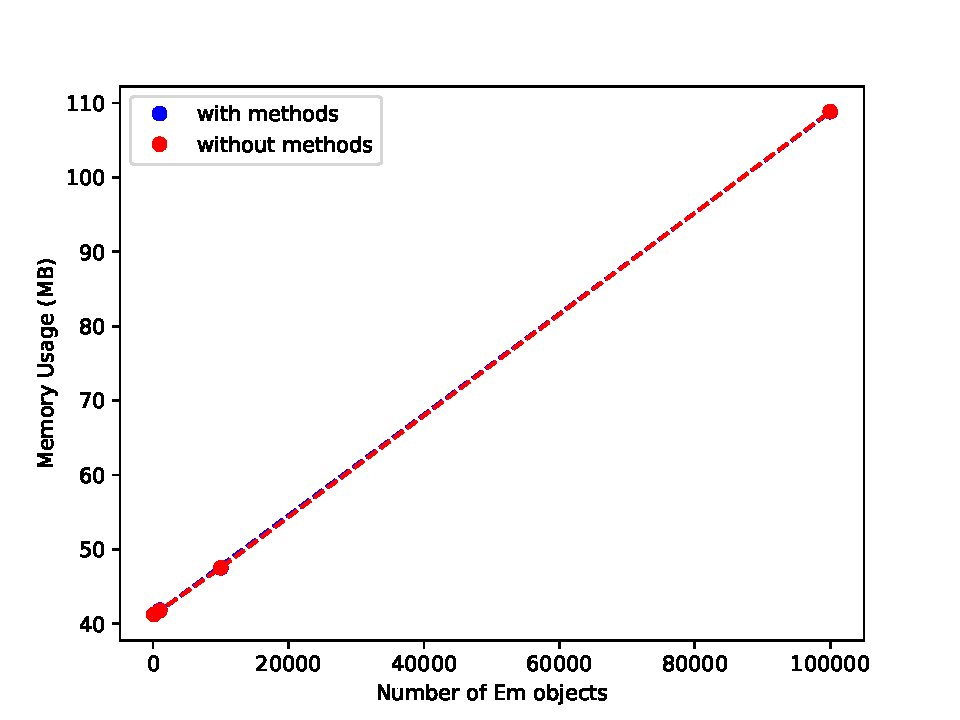
\includegraphics[height=0.8\textheight]{em_usage}
Memory usage per em with/without methods: 0.68 kB/0.68 kB
\end{center}
\end{frame}

\section{Distributed computing in Python with Ray}

\begin{frame}
\begin{itemize}
\item I looked up further information about distributed computing in Python using Ray.
\item \href{https://medium.com/formcept/scaling-python-modules-using-ray-framework-e5fc5430dc3e}{This post} and \href{https://github.com/ray-project/ray/blob/master/README.rst}{the Ray README on GitHub} seems to confirm that you can write a Python function/class to run on a single machine and then add a decorator and a few lines prior to the function call/class instantiation call to run the function asynchronously over a cluster.
\end{itemize}
\end{frame}

\section{Cartesian sampling pulses}

\begin{frame}
\begin{itemize}
\item I set the number of samples in the phase-encoding and frequency encoding directions as 11.
\item I set $k_{x, max} = k_{y,max} = 1.0~\mathrm{cm}$.
\item I used the gyromagnetic ratio of H-1.
\item See next slide for the pulses.
\end{itemize}
\end{frame}

\begin{frame}
\begin{center}
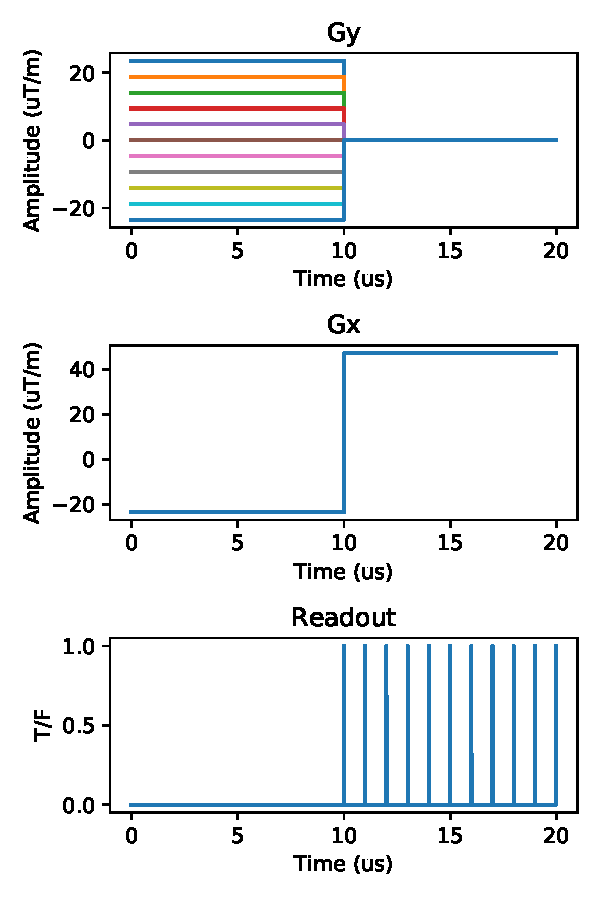
\includegraphics[height=\textheight]{kspace_pulses}
\end{center}
\end{frame}

\begin{frame}
\begin{itemize}
\item I wrote a function to compute the $k_x$ and $k_y$ samples from such a set of pulses.
\item This function returns the expected values $k_x = [-1:0.2:1]~\mathrm{cm}$ and $ky = [1:-.2:-1]~\mathrm{cm}$ when called with the pulse sequence shown above. 
\end{itemize}
\end{frame}


\end{document}